\documentclass{article}
\usepackage[T1]{fontenc}
\usepackage{lmodern}
\usepackage{graphicx}
\usepackage{amsmath,amssymb}
\usepackage[a4paper,margin=2cm]{geometry}
\usepackage[absolute,overlay]{textpos}
\setlength{\TPHorizModule}{1mm}
\setlength{\TPVertModule}{1mm}
\usepackage[indonesian]{babel}
\usepackage{hyperref}
\setlength{\emergencystretch}{2em}
% unit: Halaman 16

\begin{document}

% === Halaman 16 (python/native) ===

16

Tahun 1499, Johannes Trithemius menulis buku 

Steganographia, yang menceritakan tentang metode 

steganografi berbasis karakter

Johannes 

Trithemius

(1404-1472 )

Selanjutnya tahun 1518 dia menulis buku tentang steganografi dan kriptografi, 

berjudul Polygraphiae.

Renaissance Steganography

% deskripsi: gambar native xref 110
\noindent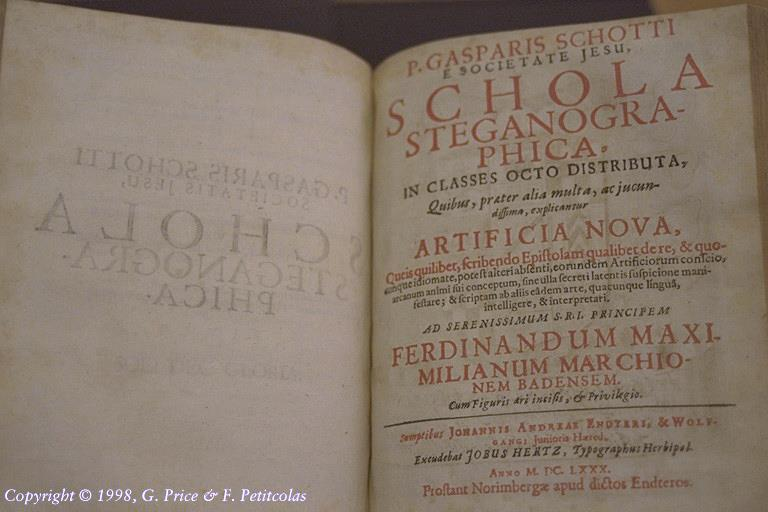
\includegraphics[width=0.85\textwidth]{../../images/python/page_016_img_01.jpeg}

% deskripsi: gambar native xref 111
\noindent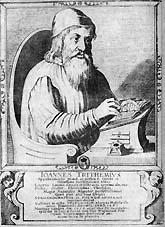
\includegraphics[width=0.85\textwidth]{../../images/python/page_016_img_02.jpeg}

% deskripsi: gambar native xref 112
\noindent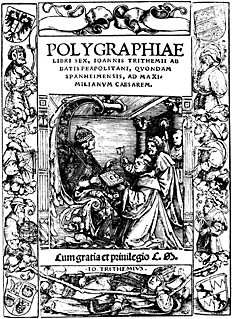
\includegraphics[width=0.85\textwidth]{../../images/python/page_016_img_03.png}

\end{document}
